\chapter{Analyse préliminaire}
\label{Chapter2}

Lors des séances préparatoires, le Prof. Olivier Donzé a décrit différentes situations réelles qui pourraient bénéficier d'une plateforme Web embarquant une visionneuse de modèles 3D avec annotations possibles, et de quelle façon celle-ci pourrait être mise à contribution.

Cela a permis d'une part d'identifier les différents groupes d'utilisateurs potentiels et leurs besoins respectifs, et d'autre part les fonctionnalités qui pourraient être mises à leur disposition. On procède donc à une analyse des besoins suivie par une analyse fonctionnelle.

\section{Besoins métiers}
\label{sec:requirements-analysis}

L'une des situations évoquées est le concours d'architecture, prenant par exemple place suite à l'adoption d'un plan localisé de quartier (PLQ)\footnote{Exemple : "Concours d'architecture sur le périmètre de la gare CEVA des Eaux-Vives" \cite{plq-contest}}.
Un tel événement regroupe les principaux acteurs de l'urbanisme, et est par conséquent une situation intéressante à analyser.

Voici une description des différentes catégories d'utilisateurs :

\textbf{Participants} \\
Pour réaliser leur projet, les participants ne partent généralement pas de rien, mais doivent prendre en compte des bâtiments et structures déjà existants. Et même si ce n'est pas le cas (zone destinée à être rasée), il faut que leur réalisation s'intègre à l'environnement avoisinant.

Une fois leur travail réalisé, celui-ci, avec d'éventuels documents annexes, doit être transmis aux personnes concernées afin d'être jugé.

\textbf{Experts} \\
Les experts effectuent une sorte de présélection, en vérifiant que les propositions répondent aux critères imposés. Ils émettent d'éventuels commentaires, à destination du jury notamment.

\textbf{Membres du jury} \\
Le jury établit le classement parmi les projets ayant passé la phase de présélection. Leur apprécation ne nécessite pas un niveau de détail aussi fourni que pour les experts. Ils peuvent adjoindre des remarques aux travaux, par exemple pour indiquer ce qui a particulièrement retenu leur attention.

\textbf{Public restreint} \\
Il s'agit d'un nombre limité de personnes "du métier", par exemple des collaborateurs du service de l'urbanisme, qui vont consulter les résultats avant que ceux-ci ne soient rendus complètement publics.
Ils peuvent ajouter des informations à destination du grand public.

\textbf{Grand public} \\
Une fois les résultats connus, une exposition est mise en place afin que la population puisse admirer les projets retenus et s'informer grâce aux informations supplémentaires mises à leur disposition.

\begin{figure}[h]
    \centering
    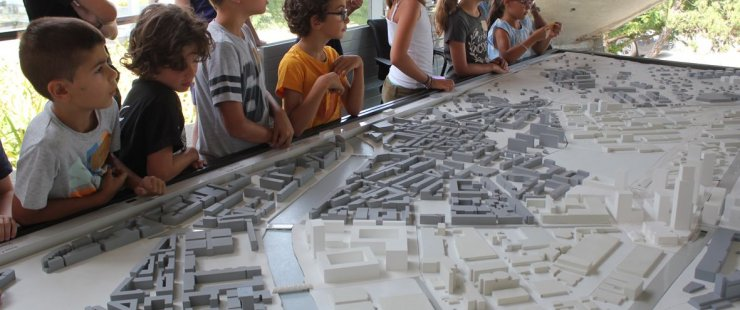
\includegraphics[width=\linewidth]{Figures/exposition-maquette-pav.jpg}
    \captionsource{Exposition de la maquette du projet Praille-Acacias-Vernets (PAV)}{pav}
    \label{fig:exposition-maquette-pav}
\end{figure}

Voici les principaux besoins qui ressortent de cette analyse:
\begin{itemize}
    \item Accéder à l'état actuel de la zone concernée (plans, maquettes...) ou au modèle sur lequel se baser. (\textit{Participants})
    \item Mettre les réalisations à disposition du comité du concours. (\textit{Participants})
    \item Consulter les modèles (\textit{Tous}, différents niveaux d'accès)
    \item Ajouter des informations au projet (\textit{Tous, excepté grand public})
    \item Consulter les informations ajoutées (\textit{Tous})
\end{itemize}

Le problème actuel est que l'accès aux informations d'origine, le rendu des projets, l'ajout de commentaires et leur communication entre les différents groupes ne sont pas toujours efficaces. De même, la consultation des modèles, comme évoqué en introduction, nécessite de savoir où, ou auprès de qui se rendre pour cela.

Pour ces raisons, un outil conçu à cet effet, accessible via le web, aurait de grands avantages.

\section{Fonctionnalités nécessaires}

Maintenant que les besoins ont été définis, il est possible d'imaginer les fonctionnalités que la plateforme pourrait offrir aux différents groupes :

\textbf{Participants} \\
Si le concours porte sur un modélisation existante, celle-ci peut leur être mise à disposition par ce biais.
Une fois réalisée, les participants déposent leurs créations sur la plateforme. On peut aussi imaginer que le système vérifie que les contraintes imposées aient été respectées, et que tous les éléments demandés aient bien été rendus.
Enfin, ils peuvent ajouter des annotations à leur modèle, par exemple pour donner plus d'information sur un élément ou joindre une photo. Ces annotations sont liées à des coordonnées spécifiques choisies.

\textbf{Experts} \\
Les experts ont un accès détaillé aux travaux des participants. Ils peuvent consulter les annotations des participants et, si nécessaire, en ajouter.

\textbf{Membres du jury} \\
Le jury a accès aux projets ayant passé la présélection. Il a accès à des fonctionnalités similaires que les experts. La vue proposée peut afficher des données plus générale que pour ces derniers.

\textbf{Public restreint} \\
Ces personnes consultent les résultats, visualisent les annotations ajoutées et peuvent en joindre d'autres, telles que des informations complémentaires sur telle ou telle "point" du modèle, destinées au grand public.

\textbf{Grand public} \\
La population peut consulter les travaux lauréats, et obtenir plus d'information en consultant les annotations associées à chacun.

Les fonctionnalités se résument ainsi :

\begin{itemize}
    \item Importation/Exportation de modèles 3D
    \item Consultation des modèles
    \item Ajout et lecture d'annotations
    \item Gestion des utilisateurs (droits d'accès)
\end{itemize}

Concernant les annotations, celles-ci visent différents buts tels que :
\begin{itemize}
    \item Un participant les utilise pour proposer des vues prédéfinies de différents points de son projet.
    \item Les experts les emploient pour émettre leurs remarques.
    \item Un membre du jury ajoute ses questions sur des points particuliers.
    \item Des annotations d'ordre général sont proposées au public.
\end{itemize}


%%%%%%% BROUILLON %%%%%%%%%%%%%%%%
Suite à cela, nous étudierons les fonctionnalités qu'il convient d'implémenter, en les décomposant par module. Nous analyserons également l'architecture générale d'une plateforme existante.

 Coggle\footnote{\url{https://coggle.it/}}, application web avec une formule gratuite également.

\begin{figure}[]
    \centering
    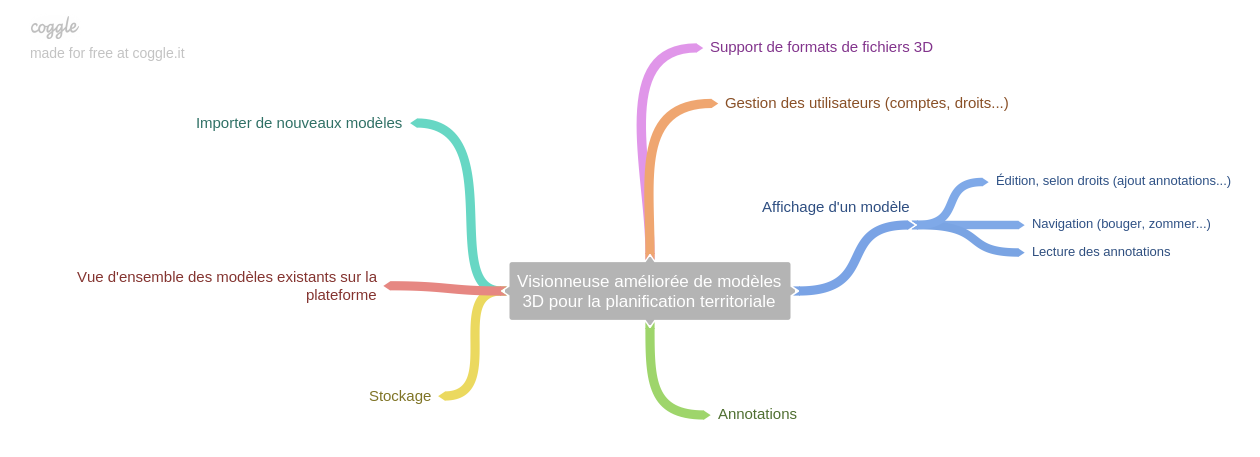
\includegraphics[width=\linewidth]{Figures/mip-viewer-mindmap.png}
    \caption{Résultat du \textit{Mind map} des modules imaginés pour l'application.}
    \label{fig:mip-viewer-mindmap}
\end{figure}

En essayant de regrouper les fonctionnalités accessibles selon le type d'utilisateur, celles-ci peuvent être résumées dans le schéma~\ref{fig:use-cases}.

\begin{figure}[ht]
    \centering
    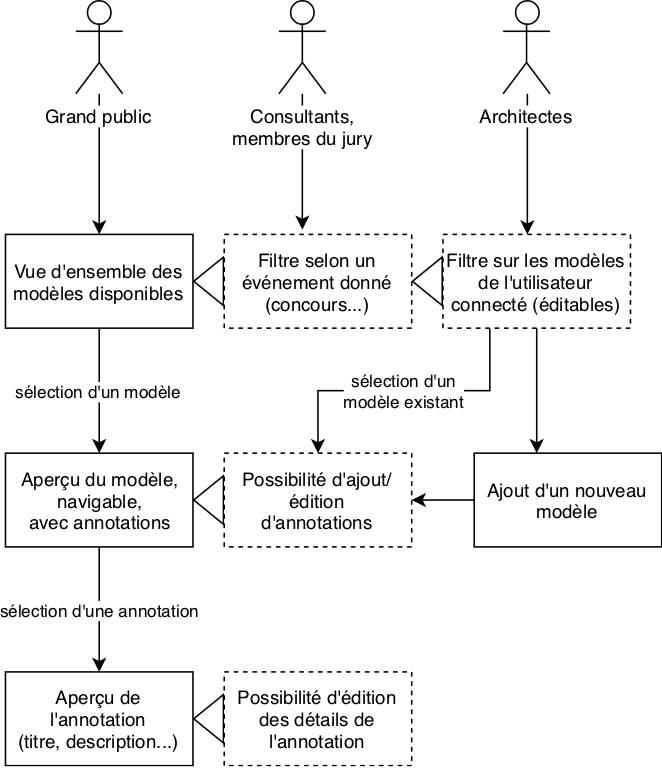
\includegraphics[width=0.8\linewidth]{Figures/use-cases.png}
    \caption{Exemples des fonctionnalités accessibles selon l'utilisateur.}
    \label{fig:use-cases}
\end{figure}






